\newpage
\section{Test und Validierung}
\label{sec:test-validation}
\begin{itemize}
	\item Testfälle beschreiben, wurden LF erfüllt?
	\item Dokumentation des Tests und der Inbetriebnahme, Testprotokoll in der Form: Erwartetes Verhalten/gemessenes Verhalten, Checklisten
	\item Genau so wie in der ES Dokumentation
\end{itemize}


\subsubsection{Testprotokoll: Latenzmessung}
\label{test-latenzmessung}

Messung der Latenz vom Zeitpunkt des Triggerinputs bis zur Audioausgabe über den Audio-Codec.

Durchführung mit dem STM32-Audioprojekt aus dem Repository (\href{run:../../f401_sd_card_audio_codec_test/}{\texttt{/f401\_sd\_card\_audio\_codec\_test/}}).
Der Audio-Codec, sowie der SD-Kartenleser müssen wie im Schaltplan(TODO: REFERENZ auf Schaltplan) verbunden werden.

\paragraph{Schritte:}
\begin{enumerate}
	\item Anschluss zweier Oszilloskop-Sonden: an Trigger-Input/Play-Button-Pin und Audio-Ausgang.
	\item Laden einer Test PCM .wav-Datei mit einer Samplerate von \SI{44.1}{\kilo\hertz}, 16 Bit und Stereo/2 Kanälen auf die SD-Karte.
	\item Umschalten des Oszilloskops in den Single-Shot-Modus und Konfiguration zur Auslösung durch den Audio-Kanal.
	\item Abspielen der Testdatei durch Auslösen des Play-Buttons.
	\item Positionierung zweier Mess-Cursor: einer auf die erste Flanke des Trigger-Input-Signals und der andere auf den Beginn des Audio-Ausgangssignals.
\end{enumerate}
\paragraph{Erwartete Werte}
	Die erwartet Latenz errechnet sich wie folgt:
	
	Gegeben:
	\begin{align*}
		\text{Samplerate} &= \SI{44.1}{\kilo\hertz} = 44{,}100 \, \text{Samples pro Sekunde} \\
		\text{Puffergröße} &= 256 \, \text{Samples}
	\end{align*}
	
	\paragraph*{Berechnung der Latenz}
	
	\[
	\text{Zeit pro Sample} = \frac{1 \, \text{Sekunde}}{44{,}100 \, \text{Samples}} \approx \SI{22.68}{\micro\second}
	\]
	
	\[
	\text{Zeit für einen Puffer} = 256 \, \text{Samples} \times \SI{22.68}{\micro\second} \approx \SI{5.8}{\milli\second}
	\]
	
	Die Latenz für ein System mit den angegebenen Parametern beträgt also etwa \( \SI{5.8}{\milli\second} \).
\paragraph{Testergebnisse}

\begin{itemize}
	\item Gemessene Latenz von \SI{6.4}{\milli\second} (\textbf{BX-AX} in Abbildung  \ref{fig:audio-latency-test}).
	\item Die Abweichung von der erwarteten Latenz ist wahrscheinlich auf die Verarbeitungszeiten des Audio-Codecs zurückzuführen sein.
	\item Sehr praktikabler Latenzwert für Audioinstrument.
\end{itemize}

\begin{figure}[H]
	\centering
	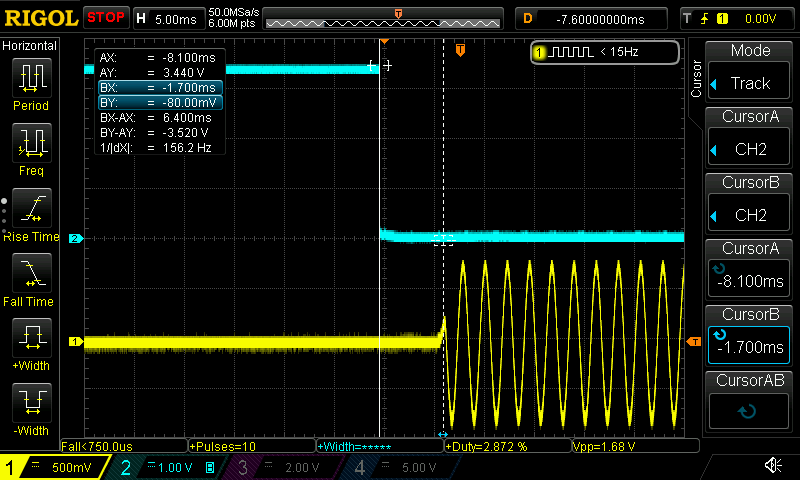
\includegraphics[width=0.6\textwidth]{images/10_test_validierung/audio/audio-latency-test.png}
	\caption{Latenzmessung von Trigger (Blau) bis Audioausgang (Gelb)}
	\label{fig:audio-latency-test}
\end{figure}



\subsection{Testprotokoll: Encoder in Verbindung mit OLED-Display}


\textcolor{red}{TODO: Tests nach Redundanz aussortieren} 

\subsubsection{Stromversorgung}
\begin{itemize}
\item \textbf{Testfall:} Überprüfung der Stromversorgung des Encoders.
\item \textbf{Schritte:}
\begin{enumerate}
\item Das System würde an eine stabile Stromquelle angeschlossen. Verbindung über einen ST-Link vom Laptop.
\item Die Spannung an den Versorgungsanschlüssen des Encoders würde mithilfe eines Multimeters gemessen.
\end{enumerate}
\item \textbf{Erwartete Werte:}
\begin{itemize}
\item Spannung: 3.3 V ± 5%.
\item Stromstärke: Im spezifizierten Bereich des Encoders.
\end{itemize}
\item \textbf{Testergebnisse:}
\begin{itemize}
\item Die gemessene Spannung betrug 3.31 V, was innerhalb des erwarteten Bereichs von 3.3 V ± 5% liegt.
\item Die Stromstärke lag ebenfalls im spezifizierten Bereich des Encoders.
\end{itemize}
\end{itemize}

\textbf{Vorgehensbeschreibung:}
Zuerst würde  das System an über ST-Link ans Laptop angeschlossen, um eine konstante Spannungsversorgung zu gewährleisten. Mit einem Multimeter würde die Spannung an den Versorgungsanschlüssen des Encoders gemessen, um sicherzustellen, dass sie im erwarteten Bereich liegt.

\subsubsection{Verbindung}
\begin{itemize}
    \item \textbf{Testfall:} Überprüfung der physischen Verbindung zwischen Encoder und Mikrocontroller.
    \item \textbf{Schritte:}
    \begin{enumerate}
        \item Die Kabelverbindungen würden mit einem Multimeter überprüft.
        \item Es würde sichergestellt, dass alle Pins korrekt verbunden sind.
    \end{enumerate}
    \item \textbf{Erwartete Werte:}
    \begin{itemize}
        \item Kontinuität und korrekte Verbindung an allen relevanten Pins.
    \end{itemize}
    \item \textbf{Testergebnisse:}
    \begin{itemize}
        \item Alle Kabelverbindungen zeigten Kontinuität.
        \item Alle relevanten Pins waren korrekt verbunden und funktionsfähig.
    \end{itemize}
\end{itemize}


\textbf{Vorgehensbeschreibung:}
Um die Verbindung zu überprüfen, haben wir zunächst ein Multimeter verwendet, um die Kontinuität der Kabelverbindungen zu testen. Die Pins des Encoders würden geprüft, um sicherzustellen, dass alle Verbindungen durchgehend und korrekt mit dem Mikrocontroller verbunden sind. Alle relevanten Pins zeigten eine korrekte Verbindung.

\subsubsection{Auswertung der Drehung des Encoders}
\begin{itemize}
    \item \textbf{Testfall:} Prüfung des Drehverhaltens
    \item \textbf{Schritte:}
    \begin{enumerate}
        \item Der Encoder würde schnell und langsam in beide Richtungen gedreht.
        \item Dabei würde die Zählvariable \texttt{rotary\_enc\_count} beobachtet.
    \end{enumerate}
    \item \textbf{Erwartete Werte:}
    \begin{itemize}
        \item Die Zählvariable zählt wie erwartet hoch und runter.
        \item Nur beim Betreten der \texttt{HAL\_GPIO\_EXTI\_Callback} soll die Variable hochgezählt werden.
    \end{itemize}
    \begin{itemize}
        \item Es traten keine Mehrfachauslösungen auf.
        \item Die Zählvariable zählte korrekt und reagierte wie erwartet auf schnelle und langsame Drehungen in beide Richtungen.
    \end{itemize}
\end{itemize}




\textbf{Vorgehensbeschreibung:}
Um das Drehverhalten des Encoders zu testen, würde de Encoder an das System angeschlossen und die Funktionalität überprüft. Anschließend haben wir den Encoder in beiden Richtungen, sowohl schnell als auch langsam, gedreht und die Zählvariable 
Die Zählvariable \texttt{rotary\_enc\_count} stand dabei unter Beobachtung, um sicherzustellen, dass sie ausschließlich durch die \texttt{HAL\_GPIO\_EXTI\_Callback} beeinflusst wird.


\subsubsection{Debouncing des Push-Buttons}
\begin{itemize}
    \item \textbf{Testfall:} Prüfung der Funktionalität des Push-Buttons.
    \item \textbf{Schritte:}
    \begin{enumerate}
        \item Drücken des Push-Button gedrückt.
        \item Prüfen ob der Interrupt korrekt ausgelöst wird.
        \item Das korrekte Verhalten des Entprellen würde geprüft.
    \end{enumerate}
    \item \textbf{Erwartete Werte:}
    \begin{itemize}
        \item Der Interrupt wird bei jedem Drücken sauber und eindeutig ausgelöst.
        \item Es treten kein Prellen oder Mehrfachauslösungen auf.
    \end{itemize}
    \item \textbf{Testergebnisse:}
    \begin{itemize}
        \item Der Interrupt wurde bei jedem Drücken zuverlässig und eindeutig ausgelöst.
        \item Es traten keine Prellen oder Mehrfachauslösungen auf.
    \end{itemize}
\end{itemize}


\textbf{Vorgehensbeschreibung:}
Der Push-Button würde mehrmals gedrückt und dabei beobachtet, ob der Interrupt korrekt ausgelöst wurde. Während des Tests wird darauf geachtet, ob der Button prellte oder Mehrfachauslösungen verursachte in dem ein Zähl Variable \texttt{cnt} im Debugger beobachte würde. Die Ergebnisse bestätigten, dass der Interrupt zuverlässig und ohne Prellen funktionierte.

\subsubsection{Menünavigation}
\begin{itemize}
    \item \textbf{Testfall:} Testen der Navigation im Menü mithilfe des Encoders.
    \item \textbf{Schritte:}
    \begin{enumerate}
        \item Den Encoder wird in beide Richtungen gedreht und die Cursor-Bewegung beobachtet. Die cursor Variable \texttt{cursor\_index} des Filemanagers würde im Debugger geprüft auf deren Zählverhalten.
        \item Der Push-Button wird gedrückt, um eine Auswahl zu treffen. Der Flag switch\_push\_button würde geprüft um die Validierung des korrekten Verhaltens beim drücken zu bestätigen.
    \end{enumerate}
    \item \textbf{Erwartete Werte:}
    \begin{itemize}
        \item Der Cursor bewegt sich entsprechend der Drehrichtung des Encoders.
        \item Die Auswahl wird korrekt angezeigt, wenn der Push-Button gedrückt wird.
    \end{itemize}

    \item \textbf{Testergebnisse:}
    \begin{itemize}
        \item Der Cursor bewegte sich korrekt und präzise entsprechend der Encoder-Drehung.
        \item Die Auswahl wurde zuverlässig angezeigt, nachdem der Push-Button gedrückt wurde.
    \end{itemize}
\end{itemize}

\textbf{Beschreibung des Vorgehens:} 
Der Encoder wird gedreht, um sicherzustellen, dass der Cursor im Menü korrekt bewegt wird. Die Cursor Variable \texttt{cursor\_index} im FileManager Struct \texttt{fm} wird korrekt hoch und runter gezählt bei entsprechender Bewegung. Anschließend habe ich den Push-Button betätigt, um zu prüfen, ob die Auswahl entsprechend angezeigt wird.  Der Flag \texttt{switch\_push\_button} würde ebenfalls korrekt gesetzt.


\subsection{Testprotokoll: Potentiometer}

\subsubsection{Verbindung überprüfen}
\begin{itemize}
    \item \textbf{Testfall:} Überprüfung der Verbindung zwischen Potentiometer und Mikrocontroller.
    \item \textbf{Schritte:}
    \begin{enumerate}
        \item Prüfung der Kabelverbindungen mit einem Multimeter.
        \item Ich habe sichergestellt, dass die Signale an den vorgesehenen Pins des Mikrocontrollers ankommen.
    \end{enumerate}
    \item \textbf{Erwartete Werte:}
    \begin{itemize}
        \item Kontinuität und korrekte Verbindung an allen relevanten Pins.
        \item Die gemessene Spannung betrug 3.29 V, was innerhalb des erwarteten Bereichs von 3.3 V ± 5% liegt.
    \end{itemize}
    \item \textbf{Beschreibung des Vorgehens:}
Die Verbindungen zwischen dem Potentiometer und dem Mikrocontroller würde überprüft, indem die Kabel mit einem Multimeter auf Kontinuität getestet habe würden. Zudem wird verifiziert, dass die Signale korrekt an den vorgesehenen Pins des Mikrocontrollers ankommen.
\end{itemize}


\subsubsection{ADC-Konfiguration überprüfen}
\begin{itemize}
    \item \textbf{Testfall:} Überprüfung der ADC-Konfiguration.
    \item \textbf{Schritte:}
    \begin{enumerate}
        \item Die Auflösung, Sample-Rate und Referenzspannung des ADCs wurden überprüft.
        \item Es wurde sichergestellt, dass der ADC korrekt konfiguriert ist.
        \item Die Referenzspannung wurde mit einem Multimeter gemessen, um ihre Übereinstimmung mit den Werte im Debugger zu bestätigen.
        \item Die Sample-Rate wurde durch Analyse der ADC-Konfigurationsregister überprüft und mit den erwarteten Werten verglichen. \texttt{ADC1\_CFGR} Configuration Register.
    \end{enumerate}
    \item \textbf{Erwartete Werte:}
    \begin{itemize}
        \item Auflösung: 12-bit (0-4096 Werte).
        \item Sample-Rate entspricht den Spezifikationen.
        \item Referenzspannung entspricht der spezifizierten Spannung.
    \end{itemize}
    \item \textbf{Testergebnisse:}
    \begin{itemize}
        \item Die Auflösung des ADCs wurde korrekt auf 12-bit (0-4096 Werte) eingestellt.
        \item Die Referenzspannung wurde mit einem Multimeter gemessen und entsprach der spezifizierten Spannung.
        \item Die Sample-Rate wurde durch Überprüfung der ADC-Konfigurationsregister bestätigt und entsprach den angegebenen Spezifikationen.
        \item Die ADC-Konfiguration war ordnungsgemäß und entsprechend den Anforderungen eingerichtet.
    \end{itemize}
\end{itemize}

\textbf{Beschreibung des Vorgehens:}
Die Konfiguration des ADCs wurde durch Überprüfung der Auflösung, Sample-Rate und Referenzspannung sichergestellt. Die Referenzspannung wurde direkt mit einem Multimeter gemessen, um ihre Übereinstimmung mit den Spezifikationen zu bestätigen. Die Sample-Rate wurde durch die Analyse der ADC-Konfigurationsregister verifiziert, indem die tatsächliche Rate mit den erwarteten Werten verglichen wurde. Die Validierung erfolgte durch den Einsatz eines Debugging-Tools, um zu gewährleisten, dass der ADC gemäß den Anforderungen konfiguriert ist.


\subsubsection{DMA-Konfiguration überprüfen}
\begin{itemize}
    \item \textbf{Testfall:} Überprüfung der DMA-Konfiguration.
    \item \textbf{Schritte:}
    \begin{enumerate}
        \item Es wurde sichergestellt, dass der DMA die ADC-Daten in den Puffer \texttt{currentValues} überträgt.
        \item Die Übertragungsart und die Übertragungsrate wurden überprüft.
        \item Das Datenformat wurde auf WORD (16-Bit) konfiguriert und geprüft.
    \end{enumerate}
    \item \textbf{Erwartete Werte:}
    \begin{itemize}
        \item Korrekte Konfiguration des DMA, Übertragungsmodus auf Circular.
        \item Datenformat korrekt auf WORD (16-Bit) eingestellt.
    \end{itemize}
    \item \textbf{Testergebnisse:}
    \begin{itemize}
        \item Der DMA überträgt die ADC-Daten wie erwartet in den Puffer \texttt{currentValues}.
        \item Die Übertragungsart ist korrekt auf Circular eingestellt.
        \item Das Datenformat wurde erfolgreich auf WORD (16-Bit) konfiguriert. Die Überprüfung wurde durch Einsicht in die DMA-Register bestätigt. Insbesondere wurden die Registerwerte für `PSIZE` und `MSIZE` auf 16-Bit überprüft, um die korrekte Einstellung des Datenformats zu bestätigen.
    \end{itemize}
\end{itemize}


\textbf{Beschreibung des Vorgehens:}
Die DMA-Konfiguration wurde überprüft, indem zuerst sichergestellt wurde, dass der DMA die ADC-Daten korrekt in den Puffer \texttt{currentValues} überträgt(Debugging). Danach wurde die Übertragungsart auf Circular gesetzt und die Übertragungsrate validiert. Schließlich wurde das Datenformat auf WORD (16-Bit) konfiguriert und durch Einsicht in die entsprechenden DMA-Register überprüft, insbesondere durch Überprüfung der Registerwerte für `PSIZE` und `MSIZE`.

\subsubsection{Daten analysieren}
\begin{itemize}
    \item \textbf{Testfall:} Analyse der aufgezeichneten ADC-Werte und Prüfung der Glättung.
    \item \textbf{Schritte:}
    \begin{enumerate}
        \item Die ADC-Werte \texttt{fm.fader\_Class[]}, \texttt{adcBuffer[]}, \texttt{smoothValue[]} und \texttt{currentClassPercentADC[]} wurden mit einem Debugger analysiert.
        \item Es wurde geprüft, ob eine lineare Zunahme der Werte entsprechend der Stellung des Schiebe-Potentiometers vorliegt.
        \item Der \texttt{smoothValue[]} wurde berechnet, und es wurde auf Schwankungen und plötzliche Änderungen geprüft. Glättung erfolgte mit \texttt{100, 1000, 10000, 30000, 100000} aufeinander addierten Werten.
    \end{enumerate}
    \item \textbf{Erwartete Werte:} 
    \begin{itemize}
        \item ADC-Werte entsprechen den Positionen des Potentiometers.
        \item Die geglätteten Werte zeigen eine stabile Wertentwicklung.
        \item Keine unerwarteten Sprünge oder signifikanten Schwankungen; Grundrauschen um wenige Volt ist normal.
    \end{itemize}
    \item \textbf{Testergebnisse:}
    \begin{itemize}
        \item Die ADC-Werte \texttt{fm.fader\_Class[]}, \texttt{adcBuffer[]}, \texttt{smoothValue[]} und \texttt{currentClassPercentADC[]} wurden erfolgreich mit dem Debugger analysiert.
        \item Die Werte zeigten eine erwartungsgemäße lineare Zunahme in Abhängigkeit von der Potentiometer-Position.
        \item Der \texttt{smoothValue[]} zeigte eine stabile Wertentwicklung ohne signifikante Schwankungen oder plötzliche Änderungen.
        \item Es traten keine unerwarteten Sprünge auf. Ein sehr geringes Grundrauschen wurde erstmal als normal eingestuft. \textcolor{red}{30000} aufeinader addierte Werte dessen Mittelwert berechnet würde stellten sich jedoch am als Effzietesten raus.
    \end{itemize}
\end{itemize}

\textbf{Beschreibung des Vorgehens:}
Die ADC-Werte wurden mit einem Debugger analysiert, um sicherzustellen, dass sie der Stellung des Potentiometers entsprechen. Es wurde überprüft, ob die Werte linear ansteigen und ob der geglättete Wert \texttt{smoothValue[]} stabil bleibt. Schwankungen und plötzliche Änderungen wurden geprüft, um die Effektivität der Glättung zu bewerten. Das Grundrauschen wurde als normal eingestuft.

\textbf{Lösung um das Grundrauschen zu minimieren:}
Das Grundrauschen könnte zukünftig durch den Einsatz von Kondensatoren, z.B. 100 nF, minimiert oder beseitigt werden.


\subsection{Testprotokoll: SD-Karten SPI-Schnittstelle}

\subsubsection{Testzielsetzung}
Dieser Test überprüft die Funktionalität der Lese- und Schreibfunktionen für die SD-Karte über die SPI-Schnittstelle.

\subsubsection{Testdurchführung}

\begin{itemize}
    \item \textbf{Mounten des Dateisystems:}
    \begin{itemize}
        \item Die Funktion \texttt{f\_mount} wurde aufgerufen, um das Dateisystem der SD-Karte zu mounten.
        \item Der Rückgabewert (\texttt{fres}) wurde überprüft. Im Fehlerfall wurde eine Meldung ausgegeben und der Test abgebrochen.
    \end{itemize}

    \item \textbf{SD-Karten-Statistiken:}
    \begin{itemize}
        \item Die Funktion \texttt{f\_getfree} wurde aufgerufen, um die freien Cluster, freien Sektoren und Gesamtsektoren der SD-Karte zu ermitteln.
        \item Im Fehlerfall wurde eine Meldung ausgegeben und der Test abgebrochen.
        \item Die Gesamt- und freien Speicherplatzwerte wurden berechnet und über \texttt{myprintf} ausgegeben.
    \end{itemize}

    \item \textbf{Lesen einer Datei:}
    \begin{itemize}
        \item Die Datei \texttt{test.txt} wurde mit der Funktion \texttt{f\_open} im Lesemodus geöffnet.
        \item Der Rückgabewert (\texttt{fres}) wurde überprüft. Im Fehlerfall wurde eine Meldung ausgegeben und der Test abgebrochen.
        \item Es wurde versucht, 30 Bytes aus der Datei zu lesen (\texttt{f\_gets}).
        \item Gelingt das Lesen, wurde der Inhalt der gelesenen Daten über \texttt{myprintf} ausgegeben.
        \item Im Fehlerfall wurde eine Meldung ausgegeben.
        \item Die Datei wurde mit \texttt{f\_close} geschlossen.
    \end{itemize}

    \item \textbf{Schreiben einer Datei:}
    \begin{itemize}
        \item Die Datei \texttt{write.txt} wurde mit der Funktion \texttt{f\_open} im Schreibmodus und mit Flags zum Anlegen der Datei geöffnet.
        \item Der Rückgabewert (\texttt{fres}) wurde überprüft. Im Fehlerfall wurde eine Meldung ausgegeben.
        \item Ein String (\texttt{"a new file is made!"}) wurde in den Puffer \texttt{readBuf} kopiert.
        \item Die Daten aus \texttt{readBuf} wurden mit \texttt{f\_write} in die Datei geschrieben.
        \item Die Anzahl der geschriebenen Bytes wurde über \texttt{myprintf} ausgegeben.
        \item Im Fehlerfall wurde eine Meldung ausgegeben.
        \item Die Datei wurde mit \texttt{f\_close} geschlossen.
    \end{itemize}

    \item \textbf{Dismounten des Dateisystems:}
    \begin{itemize}
        \item Die Funktion \texttt{f\_mount} wurde mit \texttt{NULL} aufgerufen, um das Dateisystem der SD-Karte zu dismounten.
    \end{itemize}
\end{itemize}

\subsubsection{Auswertung}
Der Test verlief erfolgreich:

\begin{itemize}
    \item Das Mounten und Dismounten des Dateisystems wurden erfolgreich durchgeführt.
    \item Die SD-Karten-Statistiken stimmten mit den Erwartungen überein.
    \item Das Lesen und Schreiben von .txt Dateien funktionierte einwandfrei.
\end{itemize}

Es wurde festgestellt, dass das Schreiben eines `struct` nicht möglich war. Eine zukünftige Lösung wird angestrebt.
